\chapter{Probabilidad}

\index{probabilidad}

Una \key{probabilidad} es un número real entre $0$ y $1$ que indica qué
tan probable es un evento. Si es evento definitivamente sucederá, su
probabilidad es 1, y si un evento es imposible, su probabilidad es 0.
La probabilidad de un evento se denota $P(\cdots)$, donde los tres
puntos describen al evento.

Por ejemplo, cuando tiramos un dado, el resultado es un entero entre
$1$ y $6$, y la probabilidad de cada resultado es $1/6$. Podemos calcular
las siguientes probabilidades, por ejemplo:

\begin{itemize}[noitemsep]
    \item $P(\textrm{``el resultado es 4''})=1/6$
    \item $P(\textrm{``el resultado no es 6''})=5/6$
    \item $P(\textrm{``el resultado es par''})=1/2$
\end{itemize}

\section{Cálculo}

Para calcular la probabilidad de un evento, podemos usar combinatoria o
simular el proceso que genere al evento. Para comenzar, calculemos la
probabilidad de sacar tres cartes con el mismo valor de un mazo de cartas
mezclado (por ejemplo, $\spadesuit\,8$, $\clubsuit\,8$, y $\diamondsuit\,8$).

\subsubsection*{Método 1}

Podemos calcular la probabilidad usando la fórmula

\[\frac{\textrm{número de resultados deseados}}{\textrm{número de resultados total}}.\]
\\
En este problema, los resultados deseados son aquellos en los que el valor
de cada carta es el mismo. Existen $13 \binom{4}{3}$ resultados tales,
porque hay $13$ posibilidades para el valor de las cartas y $\binom{4}{3}$
maneras de elegir $3$ palos de $4$ palos posibles.

Hay un total de $\binom{52}{3}$ resultados, porque podemos elegir 3 cartas
de las 52 cartas. Por lo tanto, la probabilidad del evento es

\[\frac{13 \binom{4}{3}}{\binom{52}{3}} = \frac{1}{425}.\]

\subsubsection*{Método 2}

Otra manera de calcular la probabilidad es simulando el proceso que genera
al evento. En este ejemplo, sacamos tres cartas, por lo que el proceso
consiste de tres pasos. Requerimos que cada paso del proceso sea exitoso.

Sacar la primera carta definitivamente es exitoso, porque no hay
restricciones sobre el resultado. El segundo paso es exitoso con una
probabilidad de $3/51$, porque existen 51 cartas y 3 de ellas tienen
el mismo valor que nuestra primera carta. Similarmente, el tercer paso
es exitoso con una probabilidad de $2/50$.

La probabilidad de que el proceso entero sea exitoso es de

\[1 \cdot \frac{3}{51} \cdot \frac{2}{50} = \frac{1}{425}.\]

\section{Eventos}

Un evento, en la teoría de probabilidad, puede representarse como un
conjunto \[A \subset X,\] donde $X$ contiene todos los resultados posibles
y $A$ es un subconjunto de los resultados. Por ejemplo, al tirar un dado,
los resultados son \[X = \{1,2,3,4,5,6\}.\]
Ahora, por ejemplo, el evento ``el resultado es par'' corresponde al
subconjunto \[A = \{2,4,6\}.\]

Cada resultado $x$ es asignado una probabilidad $p(x)$. Luego, la
probabilidad $p(A)$ de un evento $A$ puede calcularse como la suma de
las probabilidades de sus resultados utilizando la fórmula
\[P(A) = \sum_{x \in A} p(x).\]
Por ejemplo, cuando tiramos un dado, $p(x)=1/6$ para cada resultado $x$,
por lo que la probabilidad del evento ``el resultado es par'' es
\[p(2)+p(4)+p(6)=1/2.\]

La probabilidad total de los resultados en $X$ debe ser 1, o sea, $P(X)=1$.

Ya que los eventos en la teoría de probabilidad son conjuntos, podemos
manipularlos utilizando las operaciones de conjuntos que ya conocemos:

\begin{itemize}
    \item El \key{complemento} $\bar A$ significa que ``$A$ no sucede''.
          Por ejemplo, tirando un dado, el complemento de $A=\{2,4,6\}$ es
          $\bar A = \{1,3,5\}$.
    \item La \key{unión} $A \cup B$ significa que ``$A$ \emph{o} $B$ suceden''.
          Por ejemplo, la unión de $A=\{2,5\}$ y $B=\{4,5,6\}$ es
          $A \cup B = \{2,4,5,6\}$.
    \item La \key{intersección} $A \cap B$ significa que ``$A$ \emph{y}
          $B$ suceden''. Por ejemplo, la intersección de $A=\{2,5\}$ y
          $B=\{4,5,6\}$ es $A \cap B = \{5\}$.
\end{itemize}

\subsubsection{Complemento}

La probabilidad del complemento $\bar A$ es calculada utilizando la fórmula
\[P(\bar A)=1-P(A).\]

A veces podemos resolver un problema fácilmente usando complementos si
resolvemos el problema opuesto. Por ejemplo, la probabilidad de conseguir
por lo menos un 6 al tirar un dado diez veces es
\[1-\left(\frac{5}{6}\right)^{10}.\]

Aquí $5/6$ es la probabilidad de que el resultado de una sola tirada \emph{no}
sea seis, y $(5/6)^{10}$ es la probabilidad de que ninguna de las tiradas
sea seis. El complemento de esta es la respuesta al problema.

\subsubsection{Unión}
\index{unión}

La probabilidad de la unión $A \cup B$ se calcula con la fórmula
\[P(A \cup B)=P(A)+P(B)-P(A \cap B).\]
Por ejemplo, al tirar un dado, la unión de los eventos
\[A=\textrm{``el resultado es par''}\]
y
\[B=\textrm{``el resultado es menor que 4''}\]
es
\[A \cup B=\textrm{``el resultado es par, o menor que 4''},\]
y su probabilidad es
\[P(A \cup B) = P(A)+P(B)-P(A \cap B)=1/2+1/2-1/6=5/6.\]

Si los eventos $A$ y $B$ son \key{disjuntos}, o sea, $A \cap B$ está vacío,
la probabilidad del evento $A \cup B$ es simplemente

\[P(A \cup B)=P(A)+P(B).\]

\subsubsection{Probabilidad condicional}

\index{probabilidad!condicional}

La \key{probabilidad condicional} \[P(A | B) = \frac{P(A \cap B)}{P(B)}\]
es la probabilidad de $A$ asumiendo que $B$ sucede. Por ende, cuando
calculamos la probabilidad de $A$, solamente consideramos los resultados
que también pertenezcan a $B$.

Usando los conjuntos anteriores, \[P(A | B)= 1/3,\] porque los resultados
de $B$ son $\{1,2,3\}$, y uno de ellos es par. Esta es la probabilidad
de un resultado par si sabemos que el resultado está entre $1 \ldots 3$.

\subsubsection{Intersección}

\index{independencia}
\index{intersección}

Usando probabilidad condicional, la probabilidad de la intersección
$A \cap B$ puede calcularse con la fórmula \[P(A \cap B)=P(A)P(B|A).\]
Los eventos $A$ y $B$ son \key{independientes} si
\[P(A|B)=P(A) \hspace{10px}\textrm{y}\hspace{10px} P(B|A)=P(B),\]
lo que significa que el hecho de que $B$ suceda no cambia la probabilidad
de $A$, y vice versa. En este caso, la probabilidad de la intersección es
\[P(A \cap B)=P(A)P(B).\]
Por ejemplo, cuando sacamos una carta del mazo, los eventos
\[A = \textrm{``el palo es tréboles''}\]
y
\[B = \textrm{``el valor es 4''}\]
son independientes. Por ende el evento
\[A \cap B = \textrm{``la carta es un 4 de tréboles''}\]
sucede con la probabilidad
\[P(A \cap B)=P(A)P(B)=1/4 \cdot 1/13 = 1/52.\]

\section{Variables aleatorias}

\index{variable aleatoria}

Una \key{variable aleatoria} es un valor generado por algún proceso
aleatorio. Por ejemplo, al tirar dos dados, una variable aleatoria posible
es \[X=\textrm{``la suma de los resultados''}.\]
Por ejemplo, si los resultados son $[4,6]$ (primero tiramos un cuatro y
después un seis), entonces el valor de $X$ es 10.

Denotamos como $P(X=x)$ a la probabilidad de que el valor de una variable
aleatoria $X$ sea $x$. Por ejemplo, al tirar dos dados, $P(X=10)=3/36$,
porque el número total de resultados es 36 y existen tres maneras posibles
de obtener la suma 10: $[4,6]$, $[5,5]$ y $[6,4]$.

\subsubsection{Valor esperado}

\index{valor esperado}

El \key{valor esperado} $E[X]$ indica el valor promedio de una variable
aleatoria $X$. El valor esperado puede calcularse como la suma
\[\sum_x P(X=x)x,\]
donde $x$ recorre todos los valores posibles de $X$.

Por ejemplo, al tirar un dado, el valor esperado es
\[1/6 \cdot 1 + 1/6 \cdot 2 + 1/6 \cdot 3 + 1/6 \cdot 4 + 1/6 \cdot 5 + 1/6 \cdot 6 = 7/2.\]

Una propiedad útil de los valores esperados es su \key{linealidad}.
Esto significa que la suma $E[X_1+X_2+\cdots+X_n]$ siempre equivale a la suma
$E[X_1]+E[X_2]+\cdots+E[X_n]$. Esta fórmula se cumple incluso si las
variables aleatorias dependen entre ellas.

Por ejemplo, al tirar dos dados, la suma esperada es
\[E[X_1+X_2]=E[X_1]+E[X_2]=7/2+7/2=7.\]

Ahora consideremos un problema donde se colocan $n$ bolas aleatoriamente
en $n$ cajas, y nuestra tarea es calcular el número esperado de cajas
vacías. Cada bola tiene una probabilidad igual de ser colocada en cualquiera
de las cajas. Por ejemplo, si $n=2$, las posibilidades son las siguientes:
\begin{center}
    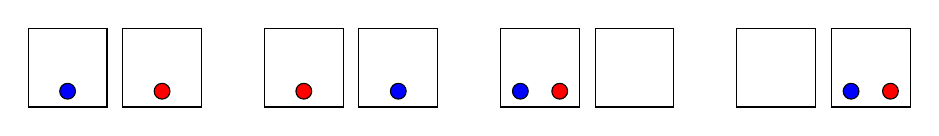
\begin{tikzpicture}
        \draw (0,0) rectangle (1,1);
        \draw (1.2,0) rectangle (2.2,1);
        \draw (3,0) rectangle (4,1);
        \draw (4.2,0) rectangle (5.2,1);
        \draw (6,0) rectangle (7,1);
        \draw (7.2,0) rectangle (8.2,1);
        \draw (9,0) rectangle (10,1);
        \draw (10.2,0) rectangle (11.2,1);

        \draw[fill=blue] (0.5,0.2) circle (0.1);
        \draw[fill=red] (1.7,0.2) circle (0.1);
        \draw[fill=red] (3.5,0.2) circle (0.1);
        \draw[fill=blue] (4.7,0.2) circle (0.1);
        \draw[fill=blue] (6.25,0.2) circle (0.1);
        \draw[fill=red] (6.75,0.2) circle (0.1);
        \draw[fill=blue] (10.45,0.2) circle (0.1);
        \draw[fill=red] (10.95,0.2) circle (0.1);
    \end{tikzpicture}
\end{center}
En este caso, el número esperado de cajas vacías es
\[\frac{0+0+1+1}{4} = \frac{1}{2}.\]
En el caso general, la probabilidad de que una caja esté vacía es
\[\left(\frac{n-1}{n}\right)^n,\]
porque ninguna bola debería colocarse en ella. Por lo tanto, usando la
linealidad, el número esperado de cajas vacías es
\[n \cdot \left(\frac{n-1}{n}\right)^n.\]

\subsubsection{Distribuciones}

\index{distribución}

La \key{distribución} de una variable aleatoria $X$ muestra la probabilidad
de cada valor que $X$ puede tomar. La distribución consiste en valores
$P(X=x)$. Por ejemplo, si tiramos dos dados, la distribución para su suma es:
\begin{center}
    \small {
        \begin{tabular}{r|rrrrrrrrrrrrr}
            $x$      & 2      & 3      & 4      & 5      & 6      & 7      & 8      & 9      & 10     & 11     & 12     \\
            $P(X=x)$ & $1/36$ & $2/36$ & $3/36$ & $4/36$ & $5/36$ & $6/36$ & $5/36$ & $4/36$ & $3/36$ & $2/36$ & $1/36$ \\
        \end{tabular}
    }
\end{center}

\index{distribución!uniforme}
En una \key{distribución uniforme}, la variable aleatoria $X$ tiene $n$
posibles valores $a,a+1,\ldots,b$ y la probabilidad de cada valor es
$1/n$. Por ejemplo, al tirar dados, $a=1$, $b=6$ y $P(X=x)=1/6$ para cada
valor $x$.

El valor esperado de $X$ en una distribución uniforme es
\[E[X] = \frac{a+b}{2}.\]

\index{distribución!binomial}
En una \key{distribución binomial}, se realizan $n$ intentos y la
probabilidad de que cada intento sea exitoso es $p$. La variable aleatoria
$X$ cuenta el número de intentos exitosos, y la probabilidad de un valor
$x$ es \[P(X=x)=p^x (1-p)^{n-x} \binom{n}{x},\] donde $p^x$ y
$(1-p)^{n-x}$ corresponde a intentos exitosos y no exitosos, y
$\binom{n}{x}$ es el número de formas en que podemos elegir el orden
de los intentos.

Por ejemplo, al tirar un dado diez veces, la probabilidad de conseguir
un seis exactamente tres veces es $(1/6)^3 (5/6)^7 \binom{10}{3}$.

El valor esperado de $X$ en una distribución binomial es \[E[X] = pn.\]

\index{distribución!geométrica}
En una \key{distribución geométrica}, la probabilidad de que un intento
sea exitoso es $p$, y continuamos hasta que el primer éxito suceda. La
variable aleatoria $X$ cuenta el número de intentos necesarios, y la
probabilidad de un valor $x$ es \[P(X=x)=(1-p)^{x-1} p,\] donde
$(1-p)^{x-1}$ corresponde a los intentos no exitosos y $p$ corresponde
al primer intento exitoso.

Por ejemplo, si tiramos un dado hasta conseguir un seis, la probabilidad
de que el número de tiradas sea exactamente 4 es $(5/6)^3 1/6$.

El valor esperado de $X$ en una distribución geométrica es
\[E[X]=\frac{1}{p}.\]

\section{Cadenas de Markov}

\index{cadena de Markov}

Una \key{cadena de Markov} es un proceso aleatorio que consiste de
estados y transiciones entre ellos. Para cada estado, sabemos las
probabilidades de movernos a otros estados. Una cadena de Markov es
representable como un grafo cuyos nodos son estados y aristas
son transiciones.

Como ejemplo, considera un problema donde estamos en el primero piso
de un edificio de $n$ pisos. En cada paso, caminamos aleatoriamente
al piso de arriba o al de abajo, excepto que siempre caminamos hacia
arriba en el piso 1 y hacia abajo en el piso $n$. ¿Cuál es la
probabilidad de estar en el piso $m$ tras $k$ pasos?

\pagebreak
En este problema, cada piso del edificio corresponde a un estado en una
cadena de Markov. Por ejemplo, si $n=5$ el grafo se ve así:

\begin{center}
    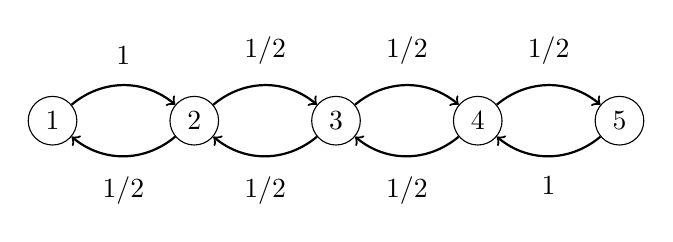
\begin{tikzpicture}[scale=0.9]
        \node[draw, circle] (1) at (0,0) {$1$};
        \node[draw, circle] (2) at (2,0) {$2$};
        \node[draw, circle] (3) at (4,0) {$3$};
        \node[draw, circle] (4) at (6,0) {$4$};
        \node[draw, circle] (5) at (8,0) {$5$};

        \path[draw,thick,->] (1) edge [bend left=40] node[font=\small,label=$1$] {} (2);
        \path[draw,thick,->] (2) edge [bend left=40] node[font=\small,label=$1/2$] {} (3);
        \path[draw,thick,->] (3) edge [bend left=40] node[font=\small,label=$1/2$] {} (4);
        \path[draw,thick,->] (4) edge [bend left=40] node[font=\small,label=$1/2$] {} (5);

        \path[draw,thick,->] (5) edge [bend left=40] node[font=\small,label=below:$1$] {} (4);
        \path[draw,thick,->] (4) edge [bend left=40] node[font=\small,label=below:$1/2$] {} (3);
        \path[draw,thick,->] (3) edge [bend left=40] node[font=\small,label=below:$1/2$] {} (2);
        \path[draw,thick,->] (2) edge [bend left=40] node[font=\small,label=below:$1/2$] {} (1);

        %\path[draw,thick,->] (1) edge [bend left=40] node[font=\small,label=below:$1$] {} (2);
    \end{tikzpicture}
\end{center}

La distribución de probabilidad de una cadena de Markov es un vector
$[p_1,p_2,\ldots,p_n]$, donde $p_k$ es la probabilidad de que el estado
actual sea $k$. La fórmula $p_1+p_2+\cdots+p_n=1$ siempre se cumple.

En la situación de arriba, la distribución inicial es $[1,0,0,0,0]$,
porque siempre comenzamos en el piso 1. La siguiente distribución es
$[0,1,0,0,0]$, porque solo podemos movernos del piso 1 al piso 2.
Luego de esto, podemos movernos hacia arriba o hacia abajo, así que
la siguiente distribución es $[1/2,0,1/2,0,0]$, y así sucesivamente.

Una manera eficiente de simular la caminata en una cadena de Markov es
utilizando la programación dinámica. La idea es mantener la distribución
de probabilidad, y en cada paso recorrer todas las posibilidades de
movimiento. Usando este método, podemos simular una caminata de $m$ pasos
en tiempo $O(n^2 m)$.

Las transiciones de una cadena de Markov también pueden representarse
como una matriz que actualiza la distribución de probabilidad. En la
situación de arriba, la matriz es

\[
    \begin{bmatrix}
        0 & 1/2 & 0   & 0   & 0 \\
        1 & 0   & 1/2 & 0   & 0 \\
        0 & 1/2 & 0   & 1/2 & 0 \\
        0 & 0   & 1/2 & 0   & 1 \\
        0 & 0   & 0   & 1/2 & 0 \\
    \end{bmatrix}.
\]

Cuando multiplicamos una distribución de probabilidad por esta matriz,
conseguimos la nueva distribución luego de dar un paso. Por ejemplo,
nos podemos mover de la distribución $[1,0,0,0,0]$ a la distribución
$[0,1,0,0,0]$ de la siguiente manera:

\[
    \begin{bmatrix}
        0 & 1/2 & 0   & 0   & 0 \\
        1 & 0   & 1/2 & 0   & 0 \\
        0 & 1/2 & 0   & 1/2 & 0 \\
        0 & 0   & 1/2 & 0   & 1 \\
        0 & 0   & 0   & 1/2 & 0 \\
    \end{bmatrix}
    \begin{bmatrix}
        1 \\
        0 \\
        0 \\
        0 \\
        0 \\
    \end{bmatrix}
    =
    \begin{bmatrix}
        0 \\
        1 \\
        0 \\
        0 \\
        0 \\
    \end{bmatrix}.
\]

Si calculamos potencias de matrices eficientemente, podemos calcular
la distribución luego de $m$ pasos en tiempo $O(n^3 \log m)$.

\section{Algoritmos aleatorios}

\index{algoritmo!aleatorio}
\indexaltsub{algoritmo}{probabilístico}

A veces podemos utilizar la aleatoriedad para resolver un problema,
incluso si el problema no está relacionado a probabilidades. Un
\key{algoritmo aleatorio} es un algoritmo que se basa en la aleatoriedad.

\index{algoritmo!Monte Carlo}

Un \key{algoritmo de Monte Carlo} es un algoritmo aleatorio que puede
devolver respuestas incorrectas. Para que un algoritmo tal sea útil,
la probabilidad de una respuesta incorrecta debe ser pequeña.

\index{algoritmo!Las Vegas}

Un \key{algoritmo de Las Vegas} es un algoritmo aleatorio que siempre
devuelve la respuesta correcta, pero su tiempo de ejecución varía
aleatoriamente. El objetivo es diseñar un algoritmo que es eficiente
con alta probabilidad.

Ahora veremos tres problemas de ejemplo que pueden resolverse
utilizando aleatoriedad.

\subsubsection{Estadísticos de orden}

\index{estatístico de orden}

El $k$-ésimo \key{estadístico de orden} de un arreglo es el elemento
en posición $k$ luego de ordenar el arreglo crecientemente. Es fácil
calcular cualquier estadístico de orden en $O(n \log n)$ si ordenamos
el arreglo, pero ¿realmente es necesario ordenar el arreglo entero
para encontrar un solo elemento?

\index{quicksort}
\index{quickselect}

Resulta que podemos encontrar estadísticos de orden utilizando un
algoritmo aleatorio sin ordenar el arreglo. El algoritmo, llamado
\key{\textit{quickselect}},\footnote{En 1961, C. A. R. Hoare publicó
    dos algoritmos eficientes en promedio: \key{quicksort} \cite{hoa61a}
    para ordenar arreglos y \key{quickselect} \cite{hoa61b} para encontrar
    estadísticos de orden.} es un algoritmo de Las Vegas: su complejidad
temporal es usualmente $O(n)$ pero $O(n^2)$ en el peor caso.

El algoritmo elige un elemento aleatorio $x$ del arreglo, y mueve los
elementos más pequeños que $x$ a la parte izquierda del arreglo, y todos
los otros elementos a la parte derecha del arreglo. Esto tarda $O(n)$
cuando hay $n$ elementos. Asumamos que la parte izquierda contiene $a$
elementos y la parte derecha contiene $b$ elementos. Si $a=k$, el
elemento $x$ es el $k$-ésimo estadístico de orden. De lo contrario, si $a>$k,
encontramos recursivamente el $k$-ésimo estadístico de orden para la
parte izquierda, y si $a<k$, encontramos recursivamente el $d$-ésimo
estadístico de orden para la parte derecha, donde $d=k-a$. La búsqueda
continúa similarmente, hasta que el elemento haya sido encontrado.

Cuando cada elemento $x$ es elegido aleatoriamente, el tamaño del arreglo
\emph{casi} se divide a la mitad en cada paso, por lo que la complejidad
temporal para encontrar el $k$-ésimo estadístico de orden es aproximadamente
\[n+n/2+n/4+n/8+\cdots < 2n = O(n).\]

El peor caso del algoritmo requiere una complejidad de $O(n^2)$, porque
es posible que $x$ siempre sea elegido de manera tal que sea uno de los
elementos más pequeños o más grandes en el arreglo y $O(n)$ pasos son
necesarios. Sin embargo, la probabilidad de que esto suceda es tan pequeña
que nunca sucede en la práctica.

\subsubsection{Verificación de multiplicación de matrices}

\index{multiplicación de matrices}

Nuestro siguiente problema es \emph{verificar} si $AB=C$ es verdadero
cuando $A$, $B$, y $C$ son matrices de tamaño $n \times n$. Por supuesto,
podemos resolver el problema si calculamos el producto $AB$ nuevamente
(en $O(n^3)$ si usamos el algoritmo básico), pero es de esperar que verificar
la respuesta fuera más fácil que calcularla desde cero.

\index{algoritmo de!Freivalds}

Resulta que podemos resolver el problema utilizando un algoritmo de
Monte Carlo\footnote{R. M. Freivalds publicó este algoritmo en 1977
    \cite{fre77}, y a veces se lo conoce como \key{algoritmo de Freivalds.}}
cuya complejidad temporal es solamente $O(n^2)$. La idea es simple:
elegimos un vector aleatorio $X$ de $n$ elementos, y calculamos las
matrices $ABX$ y $CX$. Si $ABX=CX$, reportamos que $AB=C$, y de lo
contrario reportamos que $AB \neq C$.

La complejidad temporal del algoritmo es $O(n^2)$ porque podemos calcular
las matrices $ABX$ y $CX$ en $O(n^2)$. Podemos calcular la matriz $ABX$
eficientemente si usamos la representación $A(BX)$, tal que solamente
dos multiplicaciones de matrices de tamaño $n \times n$ y $n \times 1$
son necesarias.

La desventaja del algoritmo es que hay una baja probabilidad de que
cometa un error al reportar que $AB=C$. Por ejemplo,
\[
    \begin{bmatrix}
        6 & 8 \\
        1 & 3 \\
    \end{bmatrix}
    \neq
    \begin{bmatrix}
        8 & 7 \\
        3 & 2 \\
    \end{bmatrix},
\]
pero
\[
    \begin{bmatrix}
        6 & 8 \\
        1 & 3 \\
    \end{bmatrix}
    \begin{bmatrix}
        3 \\
        6 \\
    \end{bmatrix}
    =
    \begin{bmatrix}
        8 & 7 \\
        3 & 2 \\
    \end{bmatrix}
    \begin{bmatrix}
        3 \\
        6 \\
    \end{bmatrix}.
\]
Sin embargo, en la práctica, la probabilidad de que este algoritmo
cometa un error es pequeña, y podemos disminuirla si verificamos el
resultado usando múltiples vectores aleatorios $X$ antes de reportar que
$AB=C$.

\subsubsection{Coloración de grafos}

\index{coloración}

Dado un grafo que contenga $n$ nodos y $m$ aristas, nuestra tarea es
encontrar una manera de colorear los nodos del grafo usando dos colores
tal que para por lo menos $m/2$ aristas, sus extremos tengan distintos
colores. Por ejemplo, en el grafo
\begin{center}
    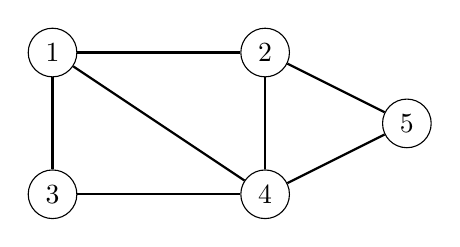
\begin{tikzpicture}[scale=0.9]
        \node[draw, circle] (1) at (1,3) {$1$};
        \node[draw, circle] (2) at (4,3) {$2$};
        \node[draw, circle] (3) at (1,1) {$3$};
        \node[draw, circle] (4) at (4,1) {$4$};
        \node[draw, circle] (5) at (6,2) {$5$};

        \path[draw,thick,-] (1) -- (2);
        \path[draw,thick,-] (1) -- (3);
        \path[draw,thick,-] (1) -- (4);
        \path[draw,thick,-] (3) -- (4);
        \path[draw,thick,-] (2) -- (4);
        \path[draw,thick,-] (2) -- (5);
        \path[draw,thick,-] (4) -- (5);
    \end{tikzpicture}
\end{center}
una coloración válida es la siguiente:
\begin{center}
    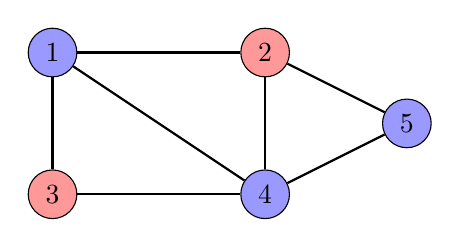
\begin{tikzpicture}[scale=0.9]
        \node[draw, circle, fill=blue!40] (1) at (1,3) {$1$};
        \node[draw, circle, fill=red!40] (2) at (4,3) {$2$};
        \node[draw, circle, fill=red!40] (3) at (1,1) {$3$};
        \node[draw, circle, fill=blue!40] (4) at (4,1) {$4$};
        \node[draw, circle, fill=blue!40] (5) at (6,2) {$5$};

        \path[draw,thick,-] (1) -- (2);
        \path[draw,thick,-] (1) -- (3);
        \path[draw,thick,-] (1) -- (4);
        \path[draw,thick,-] (3) -- (4);
        \path[draw,thick,-] (2) -- (4);
        \path[draw,thick,-] (2) -- (5);
        \path[draw,thick,-] (4) -- (5);
    \end{tikzpicture}
\end{center}
El grafo de arriba contiene 7 aristas, y para 5 de ellas, los extremos
tienen diferentes colores, así que la coloración es válida.

El problema puede resolverse utilizando un algoritmo de Las Vegas que
genera coloraciones aleatorias hasta que una válida haya sido encontrada.
En una coloración aleatoria, el color de cada nodo se elige
independientemente así que la probabilidad de ambos colores es $1/2$.

En una coloración aleatoria, la probabilidad de que los dos extremos de
una arista tengan colores distintos es $1/2$. Por ende, el número esperado
de aristas cuyos extremos tengan distintos colores es $m/2$. Debido a que
es esperado que una coloración aleatoria sea válida, en la práctica
podremos encontrar una coloración válida rápidamente.